\documentclass{ximera}

%\usepackage{todonotes}

\newcommand{\todo}{}

\usepackage{esint} % for \oiint
\ifxake%%https://math.meta.stackexchange.com/questions/9973/how-do-you-render-a-closed-surface-double-integral
\renewcommand{\oiint}{{\large\bigcirc}\kern-1.56em\iint}
\fi


\graphicspath{
  {./}
  {ximeraTutorial/}
  {basicPhilosophy/}
  {functionsOfSeveralVariables/}
  {normalVectors/}
  {lagrangeMultipliers/}
  {vectorFields/}
  {greensTheorem/}
  {shapeOfThingsToCome/}
  {dotProducts/}
  {partialDerivativesAndTheGradientVector/}
  {../productAndQuotientRules/exercises/}
  {../normalVectors/exercisesParametricPlots/}
  {../continuityOfFunctionsOfSeveralVariables/exercises/}
  {../partialDerivativesAndTheGradientVector/exercises/}
  {../directionalDerivativeAndChainRule/exercises/}
  {../commonCoordinates/exercisesCylindricalCoordinates/}
  {../commonCoordinates/exercisesSphericalCoordinates/}
  {../greensTheorem/exercisesCurlAndLineIntegrals/}
  {../greensTheorem/exercisesDivergenceAndLineIntegrals/}
  {../shapeOfThingsToCome/exercisesDivergenceTheorem/}
  {../greensTheorem/}
  {../shapeOfThingsToCome/}
  {../separableDifferentialEquations/exercises/}
  {vectorFields/}
}

\newcommand{\mooculus}{\textsf{\textbf{MOOC}\textnormal{\textsf{ULUS}}}}

\usepackage{tkz-euclide}
\usepackage{tikz}
\usepackage{tikz-cd}
\usetikzlibrary{arrows}
\tikzset{>=stealth,commutative diagrams/.cd,
  arrow style=tikz,diagrams={>=stealth}} %% cool arrow head
\tikzset{shorten <>/.style={ shorten >=#1, shorten <=#1 } } %% allows shorter vectors

\usetikzlibrary{backgrounds} %% for boxes around graphs
\usetikzlibrary{shapes,positioning}  %% Clouds and stars
\usetikzlibrary{matrix} %% for matrix
\usepgfplotslibrary{polar} %% for polar plots
\usepgfplotslibrary{fillbetween} %% to shade area between curves in TikZ
%\usetkzobj{all}
\usepackage[makeroom]{cancel} %% for strike outs
%\usepackage{mathtools} %% for pretty underbrace % Breaks Ximera
%\usepackage{multicol}
\usepackage{pgffor} %% required for integral for loops



%% http://tex.stackexchange.com/questions/66490/drawing-a-tikz-arc-specifying-the-center
%% Draws beach ball
\tikzset{pics/carc/.style args={#1:#2:#3}{code={\draw[pic actions] (#1:#3) arc(#1:#2:#3);}}}



\usepackage{array}
\setlength{\extrarowheight}{+.1cm}
\newdimen\digitwidth
\settowidth\digitwidth{9}
\def\divrule#1#2{
\noalign{\moveright#1\digitwidth
\vbox{\hrule width#2\digitwidth}}}




% \newcommand{\RR}{\mathbb R}
% \newcommand{\R}{\mathbb R}
% \newcommand{\N}{\mathbb N}
% \newcommand{\Z}{\mathbb Z}

\newcommand{\sagemath}{\textsf{SageMath}}


%\renewcommand{\d}{\,d\!}
%\renewcommand{\d}{\mathop{}\!d}
%\newcommand{\dd}[2][]{\frac{\d #1}{\d #2}}
%\newcommand{\pp}[2][]{\frac{\partial #1}{\partial #2}}
% \renewcommand{\l}{\ell}
%\newcommand{\ddx}{\frac{d}{\d x}}

% \newcommand{\zeroOverZero}{\ensuremath{\boldsymbol{\tfrac{0}{0}}}}
%\newcommand{\inftyOverInfty}{\ensuremath{\boldsymbol{\tfrac{\infty}{\infty}}}}
%\newcommand{\zeroOverInfty}{\ensuremath{\boldsymbol{\tfrac{0}{\infty}}}}
%\newcommand{\zeroTimesInfty}{\ensuremath{\small\boldsymbol{0\cdot \infty}}}
%\newcommand{\inftyMinusInfty}{\ensuremath{\small\boldsymbol{\infty - \infty}}}
%\newcommand{\oneToInfty}{\ensuremath{\boldsymbol{1^\infty}}}
%\newcommand{\zeroToZero}{\ensuremath{\boldsymbol{0^0}}}
%\newcommand{\inftyToZero}{\ensuremath{\boldsymbol{\infty^0}}}



% \newcommand{\numOverZero}{\ensuremath{\boldsymbol{\tfrac{\#}{0}}}}
% \newcommand{\dfn}{\textbf}
% \newcommand{\unit}{\,\mathrm}
% \newcommand{\unit}{\mathop{}\!\mathrm}
% \newcommand{\eval}[1]{\bigg[ #1 \bigg]}
% \newcommand{\seq}[1]{\left( #1 \right)}
% \renewcommand{\epsilon}{\varepsilon}
% \renewcommand{\phi}{\varphi}


% \renewcommand{\iff}{\Leftrightarrow}

% \DeclareMathOperator{\arccot}{arccot}
% \DeclareMathOperator{\arcsec}{arcsec}
% \DeclareMathOperator{\arccsc}{arccsc}
% \DeclareMathOperator{\si}{Si}
% \DeclareMathOperator{\scal}{scal}
% \DeclareMathOperator{\sign}{sign}


%% \newcommand{\tightoverset}[2]{% for arrow vec
%%   \mathop{#2}\limits^{\vbox to -.5ex{\kern-0.75ex\hbox{$#1$}\vss}}}
% \newcommand{\arrowvec}[1]{{\overset{\rightharpoonup}{#1}}}
% \renewcommand{\vec}[1]{\arrowvec{\mathbf{#1}}}
% \renewcommand{\vec}[1]{{\overset{\boldsymbol{\rightharpoonup}}{\mathbf{#1}}}}

% \newcommand{\point}[1]{\left(#1\right)} %this allows \vector{ to be changed to \vector{ with a quick find and replace
% \newcommand{\pt}[1]{\mathbf{#1}} %this allows \vec{ to be changed to \vec{ with a quick find and replace
% \newcommand{\Lim}[2]{\lim_{\point{#1} \to \point{#2}}} %Bart, I changed this to point since I want to use it.  It runs through both of the exercise and exerciseE files in limits section, which is why it was in each document to start with.

% \DeclareMathOperator{\proj}{\mathbf{proj}}
% \newcommand{\veci}{{\boldsymbol{\hat{\imath}}}}
% \newcommand{\vecj}{{\boldsymbol{\hat{\jmath}}}}
% \newcommand{\veck}{{\boldsymbol{\hat{k}}}}
% \newcommand{\vecl}{\vec{\boldsymbol{\l}}}
% \newcommand{\uvec}[1]{\mathbf{\hat{#1}}}
% \newcommand{\utan}{\mathbf{\hat{t}}}
% \newcommand{\unormal}{\mathbf{\hat{n}}}
% \newcommand{\ubinormal}{\mathbf{\hat{b}}}

% \newcommand{\dotp}{\bullet}
% \newcommand{\cross}{\boldsymbol\times}
% \newcommand{\grad}{\boldsymbol\nabla}
% \newcommand{\divergence}{\grad\dotp}
% \newcommand{\curl}{\grad\cross}
%\DeclareMathOperator{\divergence}{divergence}
%\DeclareMathOperator{\curl}[1]{\grad\cross #1}
% \newcommand{\lto}{\mathop{\longrightarrow\,}\limits}

% \renewcommand{\bar}{\overline}

\colorlet{textColor}{black}
\colorlet{background}{white}
\colorlet{penColor}{blue!50!black} % Color of a curve in a plot
\colorlet{penColor2}{red!50!black}% Color of a curve in a plot
\colorlet{penColor3}{red!50!blue} % Color of a curve in a plot
\colorlet{penColor4}{green!50!black} % Color of a curve in a plot
\colorlet{penColor5}{orange!80!black} % Color of a curve in a plot
\colorlet{penColor6}{yellow!70!black} % Color of a curve in a plot
\colorlet{fill1}{penColor!20} % Color of fill in a plot
\colorlet{fill2}{penColor2!20} % Color of fill in a plot
\colorlet{fillp}{fill1} % Color of positive area
\colorlet{filln}{penColor2!20} % Color of negative area
\colorlet{fill3}{penColor3!20} % Fill
\colorlet{fill4}{penColor4!20} % Fill
\colorlet{fill5}{penColor5!20} % Fill
\colorlet{gridColor}{gray!50} % Color of grid in a plot

\newcommand{\surfaceColor}{violet}
\newcommand{\surfaceColorTwo}{redyellow}
\newcommand{\sliceColor}{greenyellow}




\pgfmathdeclarefunction{gauss}{2}{% gives gaussian
  \pgfmathparse{1/(#2*sqrt(2*pi))*exp(-((x-#1)^2)/(2*#2^2))}%
}


%%%%%%%%%%%%%
%% Vectors
%%%%%%%%%%%%%

%% Simple horiz vectors
\renewcommand{\vector}[1]{\left\langle #1\right\rangle}


%% %% Complex Horiz Vectors with angle brackets
%% \makeatletter
%% \renewcommand{\vector}[2][ , ]{\left\langle%
%%   \def\nextitem{\def\nextitem{#1}}%
%%   \@for \el:=#2\do{\nextitem\el}\right\rangle%
%% }
%% \makeatother

%% %% Vertical Vectors
%% \def\vector#1{\begin{bmatrix}\vecListA#1,,\end{bmatrix}}
%% \def\vecListA#1,{\if,#1,\else #1\cr \expandafter \vecListA \fi}

%%%%%%%%%%%%%
%% End of vectors
%%%%%%%%%%%%%

%\newcommand{\fullwidth}{}
%\newcommand{\normalwidth}{}



%% makes a snazzy t-chart for evaluating functions
%\newenvironment{tchart}{\rowcolors{2}{}{background!90!textColor}\array}{\endarray}

%%This is to help with formatting on future title pages.
\newenvironment{sectionOutcomes}{}{}



%% Flowchart stuff
%\tikzstyle{startstop} = [rectangle, rounded corners, minimum width=3cm, minimum height=1cm,text centered, draw=black]
%\tikzstyle{question} = [rectangle, minimum width=3cm, minimum height=1cm, text centered, draw=black]
%\tikzstyle{decision} = [trapezium, trapezium left angle=70, trapezium right angle=110, minimum width=3cm, minimum height=1cm, text centered, draw=black]
%\tikzstyle{question} = [rectangle, rounded corners, minimum width=3cm, minimum height=1cm,text centered, draw=black]
%\tikzstyle{process} = [rectangle, minimum width=3cm, minimum height=1cm, text centered, draw=black]
%\tikzstyle{decision} = [trapezium, trapezium left angle=70, trapezium right angle=110, minimum width=3cm, minimum height=1cm, text centered, draw=black]


\title{Polynomials}

\begin{document}

\begin{abstract}
sums of power functions
\end{abstract}
\maketitle


In the world of functions, polynomials play a similar role as the integers play in the real numbers. And, if we'll confine our discuss to only continuous functions on closed intervals, then polynomials are more like the rational numbers - you can find a polynomial as close as you want to any continuous function. \\


In other words, no matter what small distance you think up...

\begin{itemize}
\item [Numbers] Given any real number, there is a rational number within that small distance of the real number.

\item [Functions] Given any continuous function on a closed interval, there is a polynomial within that ``small distance'' of the continuous function.
\end{itemize}

This makes polynomials extremely useful and thus very interesting. \\


$\blacktriangleright$ Polynomials are sums of special functions called \textbf{power functions}, so let's begin with power functions.













\section*{Power Functions}

\begin{definition} \textbf{\textcolor{green!50!black}{Power Functions}}

A power function is any function that can be represented with a formula of the form

\[   f(x) = k \, x^p      \]

where $k$ and $p$ are nonzero real numbers.

$k$ is called the \textbf{leading coefficient}.

$p$ is called the \textbf{exponent} or the \textbf{power}.


\end{definition}



We don't need all of the power functions for polynomials.  We only need power functions with whole number exponents. But let's just get a fuller picture by examining power functions with integer exponents. We'll start with the global scale.\\





\subsection*{Asymptotic and End-Behavior}



$\blacktriangleright$  When the power, $p$, is a positive integer, then power functions have two types of end-behavior.

\begin{itemize}
\item When $p$ is even, the end-behavior is the same to the right or left.


Correspondingly, both sides of the graph go up or down, depending on the sign of the coefficient, $k$.


\item When $p$ is odd, the end-behavior is opposite on either side.


Correspondingly, the two sides of the graph go up and down in opposite directions, depending on the sign of the coefficient, $k$.




\end{itemize}


\begin{image}
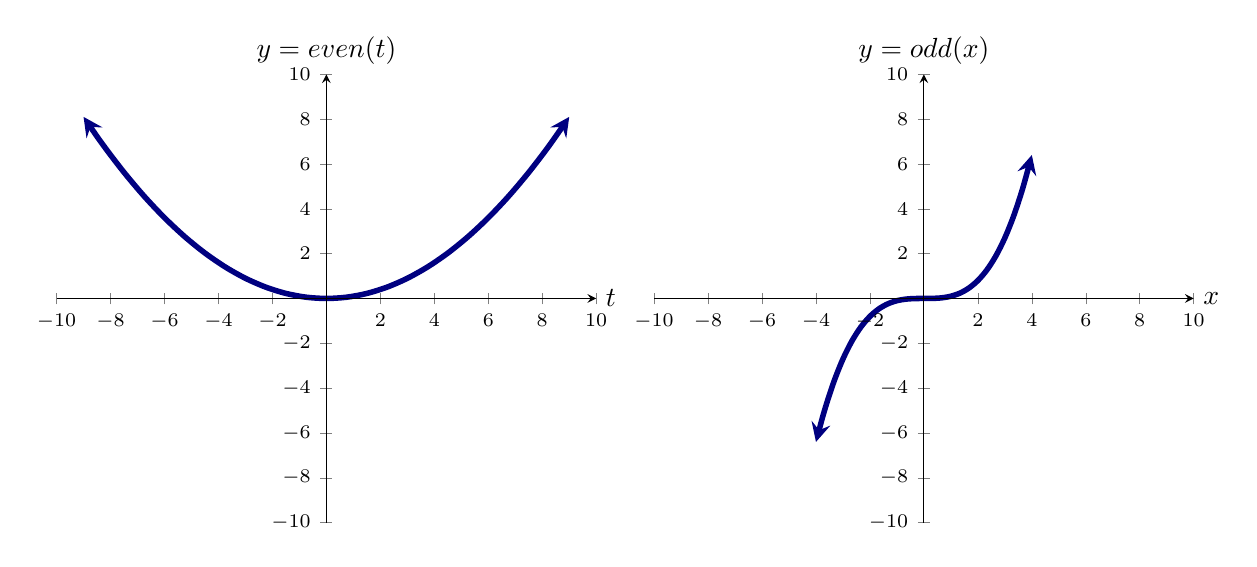
\begin{tikzpicture}
  	\begin{axis}[name = leftgraph, 
            domain=-10:10, ymax=10, xmax=10, ymin=-10, xmin=-10,
            axis lines =center, xlabel=$t$, ylabel={$y=even(t)$}, 
            ytick={-10,-8,-6,-4,-2,2,4,6,8,10},
            xtick={-10,-8,-6,-4,-2,2,4,6,8,10},
            ticklabel style={font=\scriptsize},
            every axis y label/.style={at=(current axis.above origin),anchor=south},
            every axis x label/.style={at=(current axis.right of origin),anchor=west},
            axis on top
          ]
          

          \addplot [line width=2, penColor, smooth, domain=(-9:9), <->] {0.1*x^2};


  	\end{axis}
  	\begin{axis}[at={(leftgraph.outer east)},anchor=outer west, 
            domain=-10:10, ymax=10, xmax=10, ymin=-10, xmin=-10,
            axis lines =center, xlabel=$x$, ylabel={$y=odd(x)$}, 
            ytick={-10,-8,-6,-4,-2,2,4,6,8,10},
          xtick={-10,-8,-6,-4,-2,2,4,6,8,10},
          ticklabel style={font=\scriptsize},
            every axis y label/.style={at=(current axis.above origin),anchor=south},
            every axis x label/.style={at=(current axis.right of origin),anchor=west},
            axis on top
          ]
          
     	\addplot [line width=2, penColor, smooth, domain=(-4:4), <->] {0.1*x^3};

           
  	\end{axis}
\end{tikzpicture}
\end{image}










$\blacktriangleright$  When the power, $p$, is a negative integer, then we have two types of unbounded behavior around the singularity at $0$. 

\begin{enumerate}
\item When $p$ is even, the behavior around the singularity is the same.  Depending on the sign of the coeficient, $k$, the function is unbounded positively or negatively as you get closer to $0$. \\


Correspondingly, both sides of the graph go up or down together, depending on the sign of the coefficient, $k$.




\item When $p$ is odd, the behavior around the singularity is opposite.  The function is unbounded positively one one side of $0$ and unbounded negatively on the other side of $0$. \\

Correspondingly, one side of the graph goes up and one side down, depending on the sign of the coeficient, $k$.
\end{enumerate}


\begin{image}
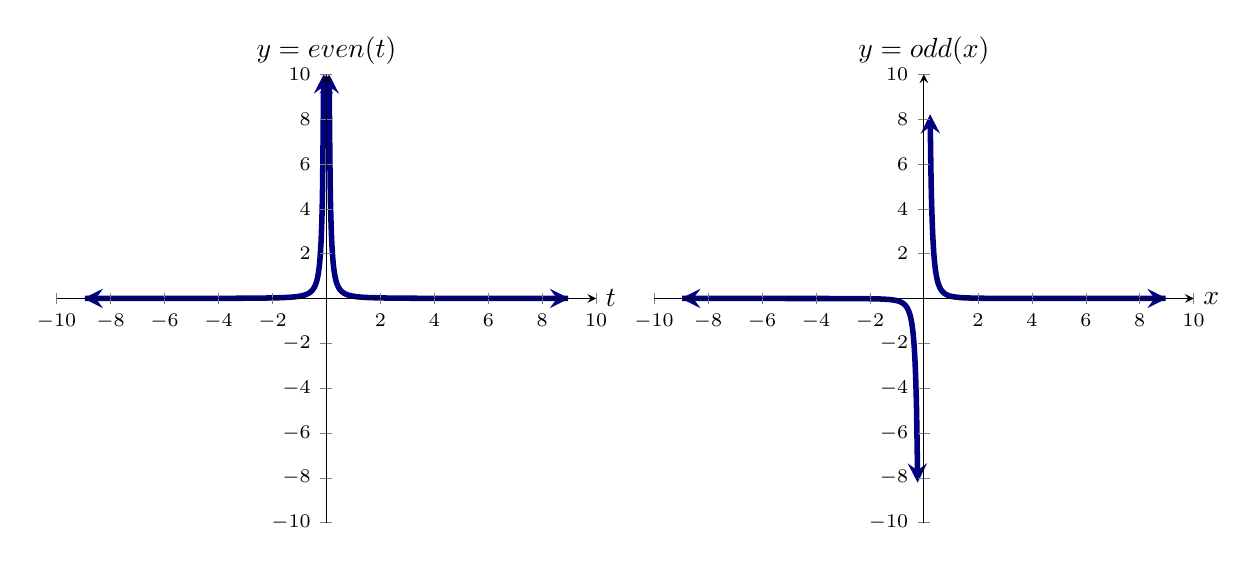
\begin{tikzpicture}
  	\begin{axis}[name = leftgraph, 
            domain=-10:10, ymax=10, xmax=10, ymin=-10, xmin=-10,
            axis lines =center, xlabel=$t$, ylabel={$y=even(t)$}, 
            ytick={-10,-8,-6,-4,-2,2,4,6,8,10},
          xtick={-10,-8,-6,-4,-2,2,4,6,8,10},
          ticklabel style={font=\scriptsize},
            every axis y label/.style={at=(current axis.above origin),anchor=south},
            every axis x label/.style={at=(current axis.right of origin),anchor=west},
            axis on top
          ]
          

          \addplot [line width=2, penColor, smooth, samples=200, domain=(-9:-0.1), <->] {0.1*x^(-2};
          \addplot [line width=2, penColor, smooth, samples=200, domain=(0.1:9), <->] {0.1*x^(-2};


  	\end{axis}
  	\begin{axis}[at={(leftgraph.outer east)},anchor=outer west, 
            domain=-10:10, ymax=10, xmax=10, ymin=-10, xmin=-10,
            axis lines =center, xlabel=$x$, ylabel={$y=odd(x)$}, 
            ytick={-10,-8,-6,-4,-2,2,4,6,8,10},
          xtick={-10,-8,-6,-4,-2,2,4,6,8,10},
          ticklabel style={font=\scriptsize},
            every axis y label/.style={at=(current axis.above origin),anchor=south},
            every axis x label/.style={at=(current axis.right of origin),anchor=west},
            axis on top
          ]
          
     	\addplot [line width=2, penColor, smooth, samples=200, domain=(-9:-0.23), <->] {0.1*x^(-3)};
     	\addplot [line width=2, penColor, smooth, samples=200, domain=(0.23:9), <->] {0.1*x^(-3)};

           
  	\end{axis}
\end{tikzpicture}
\end{image}

In either case, the end-behavior is to tend toward $0$.

















\subsection*{Limit Notation }



In the previous descriptions, our graphs did a good job of describing asymptotic and end-behavior behavior.  We would also like algebraic descriptions of these behaviors. \\


\textbf{\textcolor{blue!55!black}{$\blacktriangleright$  \textbf{End-Behavior}}} 

The domain of a power function is either all the real numbers, $\mathbb{R}$, or all of the real numbers except $0$, $\mathbb{R} \setminus \{ 0 \}$.  In either case we can imagine moving far off to the left or far off to the right on the number line to where the domain is made up of very large negative or very large positive numbers, the tail ends.  When we want the reader to think of moving even further to the right we use the phrase ``tending to infinity''. When we want the reader to think of moving even further to the left we use the phrase ``tending to negative infinity''.

For power functions with a negative power, the function values become smaller and smaller as the domain tends to positive or negative infinity.

The mathematical word for this ``tending'' relationship is \textbf{\textcolor{purple!85!blue}{limit}}.

If we inspect a power function, $f(x) = k \, x^p$, with a negative power, then we see that as $x$ tends to positive infinity, the value of $f(x)$ tends to $0$.  The algebraic way of writing this looks like


\[    \lim_{x \to \infty} k \, x^p = 0,        \]


\textbf{\textcolor{purple!85!blue}{Pronounced:}} \textit{The limit of $k \, x^p$ as x tends towards infinity equals zero}.


We also have,

\[    \lim_{x \to -\infty} k \, x^p = 0,        \]


\textbf{\textcolor{purple!85!blue}{Pronounced:}} \textit{The limit of $k \, x^p$ as x tends towards negative infinity equals zero}.


For power functions with a positive power, we have limits such as 



\[    \lim_{x \to -\infty} k \, x^p =  -\infty  \,   \text{ or }  \,  \lim_{x \to -\infty} k \, x^p =  \infty  \,   \text{ or }  \,     \lim_{x \to \infty} k \, x^p = -\infty  \,  \text{ or }  \,     \lim_{x \to \infty} k \, x^p = \infty  \]




It depends on the sign of the coefficient $k$.




\begin{notation}


Although the graph is convincing, ``we can see'' is not rigorous reasoning. \\


We would like a precise and proper explanation of $\lim_{x \to \infty} k \, x^p = 0$, when $p$ is a negative integer. \\


Let $k$ be any non-zero real number. \\
If $p$ is a negative integer, then let $p = -n$, where $n$ is a positive integer. \\
Let $f(x) = k \, x^p = \frac{k}{x^n}$ \\



For the limit to equal $0$, $f$ must ``eventually'' get smaller than any real number, and stay there. \\


Let $\epsilon > 0$ represent a very small real number.  Does $\frac{k}{x^n}$ get smaller than $\epsilon$, and stay smaller, for larger enough $x$? \\

Let's see. \\



Given any small $\epsilon > 0$, let $M = \frac{1}{| k | \cdot \epsilon}$, which is a positive real number.


For any $x > M$, we have 

\[
| f(x) | = | k | \, x^p  = \frac{| k |}{x^n} < \frac{| k |}{x} < \frac{| k |}{M}  = \epsilon
\] 


Given any small positive distance from $0$, called $\epsilon$, eventually $| f(x) |$ gets smaller and stays there. \\



The ``eventually'' part is $M$. \\

The ``stays there'' part is, for any $x > M$.


\end{notation}
















\textbf{\textcolor{blue!55!black}{$\blacktriangleright$  \textbf{Singularity Behavior}}} 



For a power function, $f(x) = k \, x^p$, with a negative power we have seen that there is a singularity at $0$, where the function value is unbounded and tends to infinity or negative infinity.  This time we want our limit notation to algebraically specify the direction we are approaching $0$.  

\begin{itemize}
\item A superscript $+$ means we are approaching from the positive side or the right side.
\item A superscript $-$ means we are approaching from the negative side or the left side.
\end{itemize}


Describing the function's behavior around $0$ with limit notation looks like




\[    \lim_{x \to 0^-} k \, x^p =  -\infty  \,   \text{ or }  \,     \lim_{x \to 0^-} k \, x^p = \infty   \,   \text{ or }  \,      \lim_{x \to 0^+} k \, x^p =  -\infty  \,   \text{ or }  \,     \lim_{x \to 0^+} k \, x^p = \infty   \]




\textbf{\textcolor{purple!85!blue}{Pronounced:}} \textit{The limit of $k \, x^p$ as x tends towards zero from the left (or right) equals infinity or negative infinity}.

It depends on the sign of coefficient $k$.



\begin{notation} \textbf{\textcolor{blue!55!black}{Limit Notation}}


Limit notation looks like

\[
\lim\limits_{x \to r} f(x) = L
\]

There are five areas.


\begin{itemize}
  \item ``lim'', which stands for limit. \\
  \item $x \to r$, which tells us the variable and the real number it is approaching.  This is written directly under ``lim''.
  \item To the left of both of those is the name of the function or its formula.  $x \to r$ does not extend under the function.  
  \item ``$=$''
  \item the limiting value or description.
\end{itemize}



\end{notation}





\begin{question}

\[ \text{Evaluate} \lim_{x \to -\infty} 3 \, x^4 \]

\begin{multipleChoice}
\choice {$-\infty$}
\choice [correct]{$\infty$}
\end{multipleChoice}
\end{question}






\begin{question}

\[ \text{Evaluate} \lim_{x \to -\infty} -5 \, x^2 \]

\begin{multipleChoice}
\choice [correct]{$-\infty$}
\choice {$\infty$}
\end{multipleChoice}
\end{question}





\begin{question}

\[ \text{Evaluate} \lim_{x \to -\infty} -5 \, x^3 \]

\begin{multipleChoice}
\choice {$-\infty$}
\choice [correct]{$\infty$}
\end{multipleChoice}
\end{question}









\begin{question}

\[ \text{Evaluate} \lim_{x \to 0^-} 3 \, x^{-4} \]

\begin{multipleChoice}
\choice {$-\infty$}
\choice [correct]{$\infty$}
\end{multipleChoice}
\end{question}




\begin{question}

\[ \text{Evaluate} \lim_{x \to 0^+} 3 \, x^{-4} \]

\begin{multipleChoice}
\choice {$-\infty$}
\choice [correct]{$\infty$}
\end{multipleChoice}
\end{question}




\begin{question}

\[ \text{Evaluate} \lim_{x \to 0^+} -3 \, x^{-4} \]

\begin{multipleChoice}
\choice [correct]{$-\infty$}
\choice {$\infty$}
\end{multipleChoice}
\end{question}




\begin{question}

\[ \text{Evaluate} \lim_{x \to 0^-} -3 \, x^{-5} \]

\begin{multipleChoice}
\choice {$-\infty$}
\choice [correct]{$\infty$}
\end{multipleChoice}
\end{question}




















\section*{Polynomial Functions}


Polynomial functions are sums of power functions with powers that are nonnegative integers (whole numbers).


\begin{definition} \textbf{\textcolor{green!50!black}{Polynomial Functions}} 

A polynomial function is any function that can be represented with a formula of the form

\[    a_n x^n + a_{n-1} x^{n-1} + \cdots + a_3 x^3 + a_2 x^2 + a_1 x^1 + a_0 x^0      \]

where the $a_k$ are real numbers and $a_n \ne 0$.

This is called the \textbf{standard form}.

$a_k$ are called \textbf{coefficients}.

$a_k x^k$ are called \textbf{terms}.



\begin{itemize}
\item $n$ is called the \textbf{degree} of the polynomial.
\item $a_n$ is called the \textbf{leading coefficient}.
\item $a_n x^n$ is called the \textbf{leading term}.
\item $a_1 x^1$ is called the \textbf{linear term}.
\item $a_0 x^0$ is called the \textbf{constant term}.
\item $x$ is called the \textbf{variable}.
\end{itemize}


\end{definition}




We almost never see polynomials written out fully like this.  Usually, we see shorthand notation.   \\



$\blacktriangleright$ \textbf{\textcolor{blue!55!black}{Polynomial Shorthand Notation}}



Let's see some shorthand notation through an example.  We'll begin with this polynomial


\[  -1 x^7 + 1 x^6 + (-1) x^5 + 0 x^4 + 0 x^3 + 5 x^2 + (-7) x^1 + 8 x^0              \]



The following shorthand notation is totally voluntary.  You are more than welcome to write this polynomial as it is written above in its proper form. However, people you work with may use the shorthand notation, so you should be familiar with it.



\begin{itemize}
\item If the leading coefficient is a $1$, then people usually do not write it. If the leading coefficient is a $-1$, then people usually just write the negative sign, $-$.


\[  -x^7 + 1 x^6 + (-1) x^5 + 0 x^4 + 0 x^3 + 5 x^2 + (-7) x^1 + 8 x^0              \]


\item If a coefficient is a negative number, then people usually change the notation to subtraction.


\[  -x^7 + 1 x^6 - 1 x^5 + 0 x^4 + 0 x^3 + 5 x^2 - 7 x^1 + 8 x^0              \]



\item If a coefficient is a $1$, then people usually do not write the $1$.


\[  -x^7 + x^6 - x^5 + 0 x^4 + 0 x^3 + 5 x^2 - 7 x^1 + 8 x^0              \]


\item If a coefficient is $0$, then people just remove the whole term.

\[  -x^7 + x^6 - x^5 + 5 x^2 - 7 x^1 + 8 x^0              \]


\item People don't write the exponent $1$.

\[  -x^7 + x^6 - x^5 + 5 x^2 - 7 x + 8 x^0              \]



\item People don't write $x^0$.

\[  -x^7 + x^6 - x^5 + 5 x^2 - 7 x + 8             \]




\end{itemize}




The last version is much shorter than the original, but they represent the exact same polynomial. You are free to use any or all of the abbreviations.\\




\begin{warning} \textbf{\textcolor{red!70!darkgray}{Rule of Shortest Expression}} 

Mathematicians don't like to write a lot.  They prefer shorter expressions.  Therefore, we are left to interpret symbols by their positions and font size and context and surrounding symbols. \\

The general rule is that you interpret the shortest expression that makes sense. \\


For instance, how to interpret $7x^5$ : is the $5$ on $x$ or $7x$?  $x$ is shorter, therefore $7x^5 = 7 (x^5)$. \\

Of course, our abbreviations and shortest expressions also cause their own confusion.

\textbf{$3+15$:} Is this $(3+1)5$ or $3+(15)$?  $5$ is shorter than $15$, however, $(3+1)5$ doesn't make sense, because there is no operator between $(3+1)$ and $5$.  On the other hand we have a shorthand abbreviation whereby no symbol means multiplication.  But that rule doesn't apply to digits.  Digits are glued together tighter than operations. $25$ never means $2 \cdot 5$. That give us $3 + 15 = 3 + (15)$. \\

Just like with any language, mathematics has its idioms.

If the shortest expression is not what you mean, then you need to use parentheses to group the symbols how you want them interpreted.

\begin{center}
\textbf{\textcolor{red!70!darkgray}{If you are unsure, then use parentheses!}} 
\end{center}


\begin{center}
\textbf{\textcolor{red!70!darkgray}{Parentheses are your friends!}} 
\end{center}


\begin{center}
\textbf{\textcolor{red!70!darkgray}{Parentheses clear up miscommunication!}} 
\end{center}



\end{warning}



\begin{question}

Write $5 x^3 + 5 x^2 + (-2) x^1 + 4 x^0$ in shorthand notation.


\[
5 x^3 + 5 x^2 - \answer{2} x + 4  
\]

\end{question}





\begin{question}

Write $(-1) x^3 + 0 x^2 + (-3) x^1 + 6 x^0$ in shorthand notation.


\begin{multipleChoice}
\choice {$-x^3 + 0 x^2 + (-3) x^1 + 6 x^0$}
\choice {$-x^3 - 3 x^1 + 6 $}
\choice [correct]{$-x^3 - 3 x + 6 $}
\choice {$-x^3 - 3 x^1 + 6 x^0$}
\end{multipleChoice}

\end{question}










\subsection*{Products vs. Sums}


We engage in two very different investigations involving polynomials.  One is an algebraic investigation and the other is our investigation - an analytic investigation.  Polynomials are functions for us and we are interested in analyzing them as functions.  This means, among other features, we are interested in their zeros.  For this, and other reasons, we prefer to write polynomials in factored form.



Rather than a sum (standard form)

\[   f(x) = a_n x^n + a_{n-1} x^{n-1} + \cdots + a_3 x^3 + a_2 x^2 + a_1 x^1 + a_0 x^0      \]

we would prefer a product (factored form)

\[   f(x) = a (x-r_n)(x-r_{n-1})  \cdots (x-r_2)(x-r_1)  \]





Unfortunately, we will need complex numbers to ALWAYS get a product of linear factors.  We only have the real numbers for this class and the best we can do is a mixture of linear and quadratic factors.



\begin{theorem} \textbf{\textcolor{green!50!black}{Fundamental Theorem of Algebra}}

When restricted to real numbers, every polynomial with real coefficients can be factored into a product of linear and irreducible quadratic factors over the real numbers.

\end{theorem}


Irreducible quadratics means they need complex numbers to factor - the discriminant of the quadratic formula is negative. \\



The theorem says that every polynomial does have such a factorization, but it does not tells us how to obtain it.  We are on our own for that, which means we need lots of practice factoring polynomials.

When analyzing polynomial functions, our first step is going to be to factor it.







\begin{question}

Write $2y^2-5y-3$ in factored form, i.e. as a product.



\begin{multipleChoice}
\choice {$(y-3)(2y-1)$}
\choice {$(y+3)(2y+1)$}
\choice [correct]{$(y-3)(2y+1)$}
\choice {$(y+3)(2y-1)$}
\end{multipleChoice}

\end{question}




























\subsection*{Graphs}




Polynomial functions are continuous everywhere (all real numbers).  Their graphs are smooth wavy curves with hills and valleys.



\begin{example}


The graph of $y = f(x) = \frac{1}{100} x^3 + \frac{1}{25} x^2 - \frac{31}{100} x - \frac{7}{10}$


\begin{image}
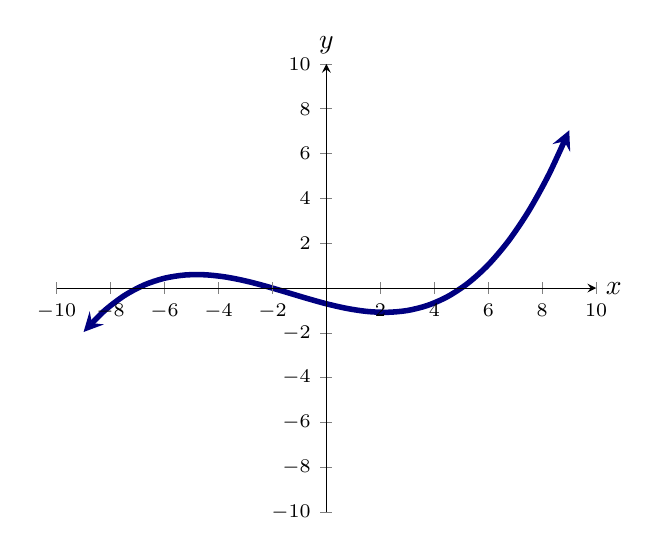
\begin{tikzpicture} 
  \begin{axis}[
            domain=-10:10, ymax=10, xmax=10, ymin=-10, xmin=-10,
            axis lines =center, xlabel=$x$, ylabel=$y$,
            ytick={-10,-8,-6,-4,-2,2,4,6,8,10},
            xtick={-10,-8,-6,-4,-2,2,4,6,8,10},
            ticklabel style={font=\scriptsize},
            every axis y label/.style={at=(current axis.above origin),anchor=south},
            every axis x label/.style={at=(current axis.right of origin),anchor=west},
            axis on top
          ]
          
          \addplot [line width=2, penColor, smooth, domain=(-9:9),<->] {0.01*(x+7)*(x+2)*(x-5)};

           

  \end{axis}
\end{tikzpicture}
\end{image}





\begin{question}

\[   \lim_{x \to -\infty} f(x)  = \infty   \]



\begin{multipleChoice}
\choice {True}
\choice [correct]{False}
\end{multipleChoice}

\end{question}



\begin{question}

\[   \lim_{x \to \infty} f(x)  = \infty   \]



\begin{multipleChoice}
\choice [correct]{True}
\choice {False}
\end{multipleChoice}

\end{question}





\end{example}








\begin{example}


The graph of $y = g(t) = \frac{1}{100} (t+7) (t+2) (t-2) (t-4) $


\begin{image}
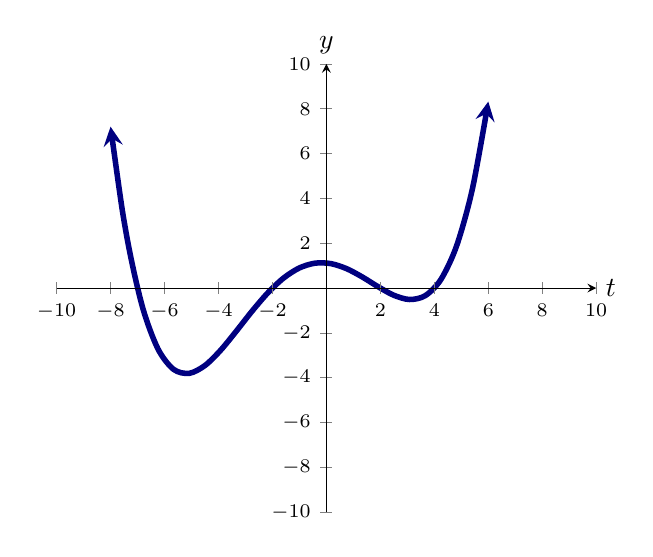
\begin{tikzpicture} 
  \begin{axis}[
            domain=-10:10, ymax=10, xmax=10, ymin=-10, xmin=-10,
            axis lines =center, xlabel=$t$, ylabel=$y$,
            ytick={-10,-8,-6,-4,-2,2,4,6,8,10},
            xtick={-10,-8,-6,-4,-2,2,4,6,8,10},
            ticklabel style={font=\scriptsize},
            every axis y label/.style={at=(current axis.above origin),anchor=south},
            every axis x label/.style={at=(current axis.right of origin),anchor=west},
            axis on top
          ]
          
          \addplot [line width=2, penColor, smooth, domain=(-8:6),<->] {0.01*(x+7)*(x+2)*(x-2)*(x-4)};

           

  \end{axis}
\end{tikzpicture}
\end{image}





\begin{question}

\[   \lim_{t \to -\infty} g(t)  = \infty   \]



\begin{multipleChoice}
\choice [correct]{True}
\choice {False}
\end{multipleChoice}

\end{question}



\begin{question}

\[   \lim_{t \to \infty} g(t)  = \infty   \]



\begin{multipleChoice}
\choice [correct]{True}
\choice {False}
\end{multipleChoice}

\end{question}




\end{example}


Polynomials have no discontinuities or singularities.  Polynomial functions may have many local maximums and minimums. They may have a global maximum or global minimum.  The only way a polynomial can have both a global maximum and a global minimum is for the polynomial to be a constant function. \\







\begin{question}

In the example above, $g(t)$ has a global minimum value.



\begin{multipleChoice}
\choice [correct]{True}
\choice {False}
\end{multipleChoice}

\end{question}



\begin{question}

In the example above, $g(t)$ has a global maximum value.



\begin{multipleChoice}
\choice {True}
\choice [correct]{False}
\end{multipleChoice}

\end{question}










\subsection*{End-Behavior}


The end-behavior of a polynomial function is the same as the leading term (a power function), which depends on the sign of the leading coefficient.











\begin{question}

Evaluate $\lim\limits_{t \to -\infty} 4 t^3 - 9 t + 3$


\begin{multipleChoice}
\choice [correct]{$-\infty$}
\choice {$\infty$}
\end{multipleChoice}

\end{question}







\begin{question}

Evaluate $\lim\limits_{t \to \infty} -4 t^3 - 5 t + 2 t^4  - 3$


\begin{multipleChoice}
\choice [correct]{$-\infty$}
\choice {$\infty$}
\end{multipleChoice}

\end{question}










\subsection*{Power-Like Functions}

We prefer writing polynomials as products, because we can quickly identify their zeros.  Products will also help us quickly determine behavior of the polynomial.

Inside the factorization

\[   f(x) = a (x-r_n)(x-r_{n-1})  \cdots (x-r_2)(x-r_1)  \]

we may have duplicate factors.

To help our analysis, it will help to gather common factors and make the factorization look like

\[   f(x) = a (x-r_n)^{e_n}(x-r_{n-1})^{e_{n-1}}  \cdots (x-r_2)^{e_2}(x-r_1)^{e_1}  \]

with all of the roots distinct, i.e. $r_k \ne r_j$ when $i \ne j$.



Analyzing polynomials will mean analyzing expressions like $(x-r_k)^{e_k}$, which looks a lot like a power function - a shifted power function.

Everything we said about power functions around $0$ holds for these shift power functions around $r_k$. 


If we think of $x^k$ as $(x-0)^k$, then $(x-r_k)^{e_k}$ seems just like a power function, just written in terms of $x-r_k$.















\begin{center}
\textbf{\textcolor{green!50!black}{ooooo-=-=-=-ooOoo-=-=-=-ooooo}} \\

more examples can be found by following this link\\ \link[More Examples of Elementary Functions]{https://ximera.osu.edu/csccmathematics/precalculus1/precalculus1/elementaryLibrary1/examples/exampleList}

\end{center}





\end{document}
